\documentclass[twocolumn]{article}
\usepackage{graphicx}
\usepackage{float}


% Will make renaming easier
\usepackage{nth}
\usepackage{xspace}
\newcommand{\projectName}{CircGraph\xspace}

\usepackage[backend=biber,url=false,doi=true]{biblatex}
\addbibresource{crosby.bib}
\usepackage{hyperref}
\usepackage{cleveref}

% We need a nicer name... todo later. Just needs to be a bit sexier for the users.
\title{\projectName: an Intelligent Galaxy Interface for Circos-enabled Genomic Data Visualization}
\author{Stephen Crosby}

\begin{document}
\maketitle
\section*{Abstract}
Advancements in molecular biology in the past two decades have led to the acquisition of
unprecedented amounts of DNA sequencing data, but the visualization of this data and its
interpretation remain incompletely solved problems in the scientific community. Several approaches to
create informative plots of sequence data have been devised in response to these challenges,
including Circos \cite{circospaper}, a configuration-file driven piece of graphics software which allows users to design circular plots highlighting
interesting genomic features and comparing different organismal genomes. Unfortunately, Circos has an extremely steep learning curve.
In order to facilitate sequence analyses for the mere mortal, a web interface to the tool interface was developed for the Galaxy \cite{galaxypaper} genomics platform.
This tool interface will enable scientists to incorporate bioinformatics visualization techniques into their work while circumventing the learning curve associated with command-line Circos usage. The tool, which has both command-line and web-based interfaces, allows users broad cosmetic control over the appearance of produced Circos plots, includes methods for parsing and interpreting several common bioinformatics-associated file formats, and supports most the principal track types present in the Circos suite. This new interface to the existing Circos software will enable life scientists to easily and efficiently create informative views of a variety of sequence data formats.

\section*{Introduction}
Macromolecular sequencing has been the underpinning of many crucial developments in modern biomedical research, and since the advent of sequencing technology in the 1970s, improvements in experimental techniques have enabled scientists to produce ever-increasing amounts of sequence data.\cite{Baker2010,Zhang2011}
The increasing popularity of these high-throughput molecular techniques has challenged the bioinformatic community to develop new solutions for data-management, statistical analysis, and genome annotation. Visualizing this newly produced genomic data remains an important obstacle to both the effective utilization of sequence data as well as the continued growth and adoption of bioinformatic methods by new scientists. Effectively managing the scale at which sequence data are visualized is critical to forming insightful conclusions, as biologically interesting genomic phenomena can occur anywhere from the single-codon up to the pangenome level. Visualization efforts are fraught with other problems as well; the emergence of new file formats to handle increasing amounts of data necessitates constant development and support to ensure existing applications retain their utilities.\cite{challenge} % cite things once per paragraph is fine. Per-sentence citations when they're all the same citation is not useful.

Naturally, a wide variety of visualization software has been produced as sequencing efforts have grown simultaneously more popular and successful; these programs in general represent sequence data as a variety of separate, static windows depicting linear chromosomes joined together by linear links indicating homologous regions as well as classic visualization options like line plots and tables, and they vary highly in their usability and quality of produced graphics. A common feature amongst these programs is to use color to encode numerical information about the uncertainty of the identity of a nucleotide within a genome and thereby maximize the information density of a single view. These software offer different options for scaling and filtering of data in order to address the difficulties heretofore described.\cite{challenge} Of the several tools built in response to the challenge of visualization, one of the most successful has been Circos: a software suite producing circular analogs of classical graphics, facilitating the comparison of genomes with compact, information-dense, two-dimensional data tracks and links. % wasn't in love with the removed sentence here, low information content.
Although the software has been successfully used to produce figures in leading scientific journals, and in its pioneering study was applied to genomic datasets spanning several orders of magnitude (kbp to Gbp), the creators of the software caution that figure quality is closely associated with aesthetic decisions made by scientists deciding which data they seek to convey, indicating that the software still has room for improvement as an exploratory visualization tool. Other visualization tools such as Circoletto, which pairs the Circos visualization paradigm with BLAST sequence identity results, have attempted to improve on Circos' visualization capabilities.\cite{circoletto} %nice.

Beyond the difficulties intrinsic to the analysis of this newly obtained high-throughput data, another obstacle to the growth of bioinformatics within classical scientific disciplines is the learning curve associated with the use of these new, computerized tools; \nth{21} century software development initiatives such as the Galaxy Project are lowering the barriers between established wet-lab scientists and cutting edge computational techniques by eschewing the traditional command-line interface in favor of broadly-accessible, user-friendly web applications.\cite{galaxypaper} % this sentence is a bit of a mouthful, but otherwise fine as-is
A wide variety of bioinformatics tools and workflows have been made publicly available in the wake of the discpline's increasing popularity, and open-source tools present low financial barriers to life scientists in academia. However, much open-source software is tailored to power users on more esoteric *NIX operating systems with a great deal of command line experience. These individuals make up only a small subset of the total potential userbase for new analytics software, highlighting the need for solutions which support a larger swath of their potential user-base, in terms of a wide variety of operating systems and shallower learning curve. An assortment of online services have been developed in order to address this issue and improve the accessibility of bioinformatics software to the scientific community at large. The Galaxy Project is just such an answer to many of the inherent problems. By providing a standardized web-interface with a collection of bioinformatics tools administrated by the global bioinformatics community, the Galaxy Project is able to provide wide accessibiltiy to an otherwise restricted discipline.\cite{galaxypaper} At the time of writing, the Galaxy Tool Shed contains over 3000 free, accessible bioinformatics tool interfaces.\cite{martin-ts} The central initiative of the Galaxy Project -- to put bioinformatics software in the hands of capable scientists with the expertise to ask difficult questions and make subtle inferences about genomic data -- was the principal factor motivating the development of \projectName.\cite{galaxypaper} The \projectName Galaxy tool replicates much of the core functionality of the Circos software suite, but hides it behind user-friendly support for parsing common data types, allowing scientists to tell the tool generally what they want, leaving the messy details of Circos configuration up to the software. Its main contribution to the body of scientific knowledge is that the program will make the existing Circos software more readily accessible to life scientists by creating Circos plots automatically from a point-and-click user interface.


\section*{Methods}
Developed in 2004, the Circos visualization software suite manages the creation of circular plots of genomic datasets using text-based configuration files; with a custom, non-standard file format similar to the text based XML format, configuration files have the potential to be automatically generated developing a software interface. A Circos configuration file is composed of blocks which represent objects ranging from heatmaps and scatterplots to position- and parameter-dependent formatting rules. Within the blocks are parameters specifying cosmetic options and indicating the data files with which data-dependent tracks will be populated. Beyond these ordinary parameters, objects can be customized by user-created rules. These rules, which rely on Perl code inserted directly into the configuration file, conditionally modify parameter values and vastly expand user control over the final diagram, allowing for advanced plotting capabilities such as mapping analysis scores directly to plot colors. \cite{circospaper}

A Galaxy tool was developed, through which users can specify data to be used in tracks and cosmetic parameters for the Circos plots. In order for the underlying tool to be widely accessible for future development, the Python programming language and the Python templating library Jinja2 were leveraged. The program manages the input parameters and transforms them to configuration files consistent with the Circos specification. Currently, the \projectName workflow is a two-stage process in which a user specifies options and quickly generates a template xml file to be passed to a command-line interface. At the command line, the user specifies data files and parameters relevant to link creation and then must manually call Circos in order to produce diagrams. Plans are in place to further refine this into a one-step ``push-button'' type workflow where the user immediately receives a Circos plot as an output.

\section*{Results and Discussion}

In order to facilitate the visualization of high-throughput genomic data in several file formats, \projectName, a web-based Galaxy tool exploiting the existing Circos software suite freely available online, was developed. The tool has implemented a significant number of features and will be publicly available within the next year. % Removed sentence saying it is command line only, no one wants to hear that.

\begin{figure}
\centering
%\includegraphics[scale=0.1]{./results/hilite.png}
\includegraphics[scale=0.15]{./results/hilite-detail.png}
\caption{\projectName allows users to create several native Circos data track types, including histograms, heatmaps, and scatterplots. Highlights can also be added to accentuate certain regions; here, highlights are shown in grey.\label{fig:hilite}}
\end{figure}


\projectName can accept and parse several common genomic file types including fasta, bigWig, gff3, and XMFA formatted multiple genome alignment files into tracks suitable for display by Circos. In particular, fasta files are used to drive the creation of the ``karyotype'' configuration and specify the chromosomes to be represented in the plots, while bigWig files are parsed into two-dimensional data tracks such as heatmaps, histograms, or scatterplots. The current Circgraph implementation does not capture the full complexity of the gff3 datatype but can parse feature locations into highlights. Alignments in general are best represented by ``links'' within the Circos visualization scheme, and consequently, XMFA files containing multiple sequence alignments are parsed into link files that illustrate connections between regions of sequence homology.

Prior to processing each of the aforementioned datatypes, lower level configuration options are exposed for each of the data tracks. This permits track customization with a wide variety of cosmetic parameters such as dictating the scales of the objects to be represented as well as their orientations, colors, and relative positions within the Circos figure.

\begin{figure}
\centering
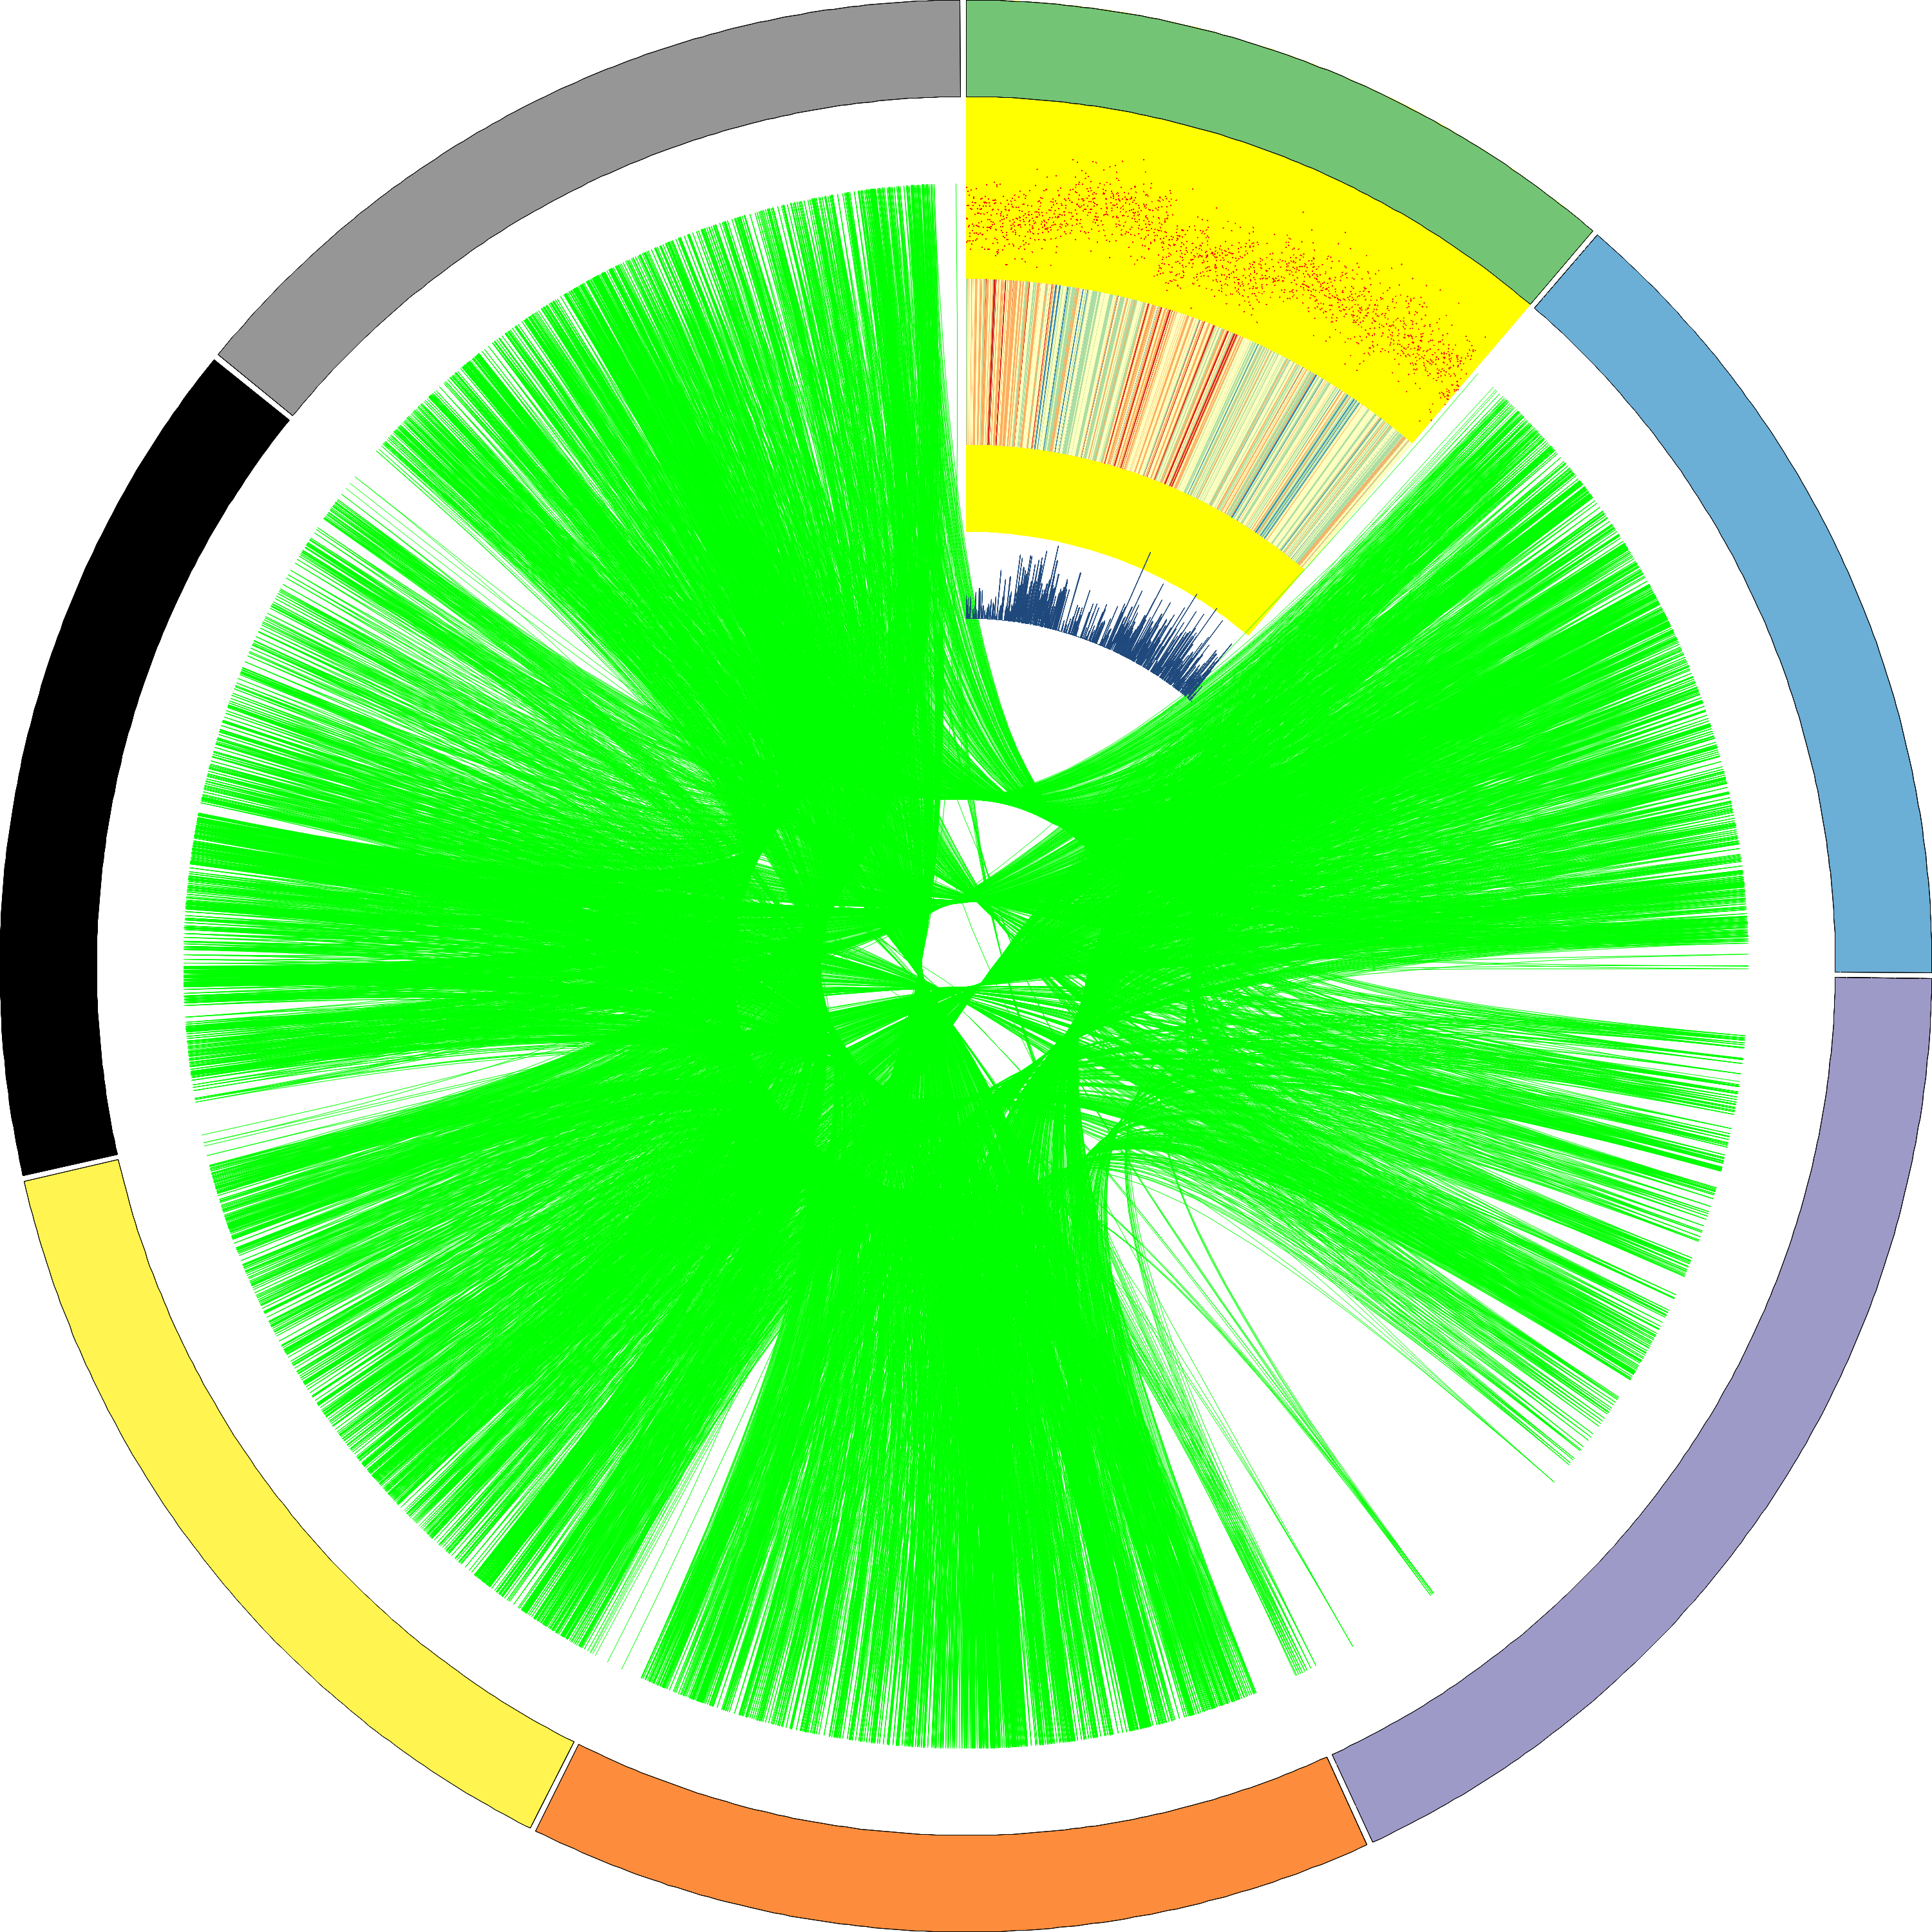
\includegraphics[scale=0.3]{./images/thumbs/links.png}
\caption{\projectName supports arrangement of multiple chromosomes within a plot and can create links between chromosomes if provided with ProgressiveMauve-generated backbone files.\label{fig:links}}
\end{figure}

Several challenges remain to the effective use of Circos for genomic data visualization; in particular, continuing improvements to existing algorithms and workflows which can separate statistically-significant, biologically-relevant data from the ambient dataset will improve the signal-to-noise ratio of Circos plots. Aside from the two-dimensional data tracks, links are the principal representative element of a Circos diagram and suggest homology between sections of the organismal genome. While proposing to maximize the ``information-to-ink''\cite{tufte} ratio of a genomics figure, the Circos software suite cannot compensate for an entirely naive approach to bioinformatics analysis; cluttered diagrams can prevent scientists from drawing inferences (\cref{fig:nonribbon}) or could even mask the data itself (\cref{fig:colorfixes}).\cite{circospaper} Although internal parameters and extensive user customization with the use of rules can enable scientists to create compelling narratives from computational analyses, determining the extent to which data supports a particular narrative, if any, is the principal problem associated with genomics visualization. Whether these analytical judgements can be made without the scientist's supervision is a question that remains to be answered. We believe with iterative refinement and improvements to the \projectName tool based on real-world usage scenarios, we can approach that goal.

\begin{figure}
\centering
\includegraphics[scale=0.3]{./images/thumbs/Generated_Data_Non_Ribbon.png}
\caption{Even when color-coded, unstratified link data is not suitable for creating easily interpreted graphics. Interpretation of this graphic with no context is a significant difficulty. Currently, \projectName does not support rules for data stratification as the graphic is being created.\label{fig:nonribbon}}
\end{figure}

\begin{figure}
\centering
\includegraphics[scale=0.4]{./images/thumbs/Generated_Color_Fixes.png}
\caption{Coarser link data poses its own interpretive difficulties; larger, opaque ribbon links can obscure each other.\label{fig:colorfixes}}
\end{figure}

Continued development of \projectName will be required in order to capture the full span of features offered by the Circos visualization software, with the end goal being guided, intelligent creation of high-quality graphics with additional user-friendliness improvements. This edition of \projectName includes several data plotting capabilities, but the inclusion of rules -- single lines of Perl code which dictate formatting on the fly based on the contents of data files -- greatly compounds the customizability of graphs the software can produce. Incorporating these dynamic formatting options into the \projectName tool without introducing a programming learning curve will be a challenge going forward; either \projectName only supports a subset of Circos' capabilities, or we overwhelm the users and induce a steeper learning curve even for our simple Galaxy interface. Either option unnecessarily limits the types of questions scientists could use the software to answer. Additionally, although elements of the software allow users to view their data at different scales are in the process of being implemented, no exploration of the effects varying scale could have on interpretability has been done. Automatic detection of sensible formatting options and determination of the optimal scale at which the data should be visualized are issues which could be addressed alongside the addition of more extensive Circos features in subsequent releases of the \projectName Galaxy tool.

\printbibliography

\end{document}
